\documentclass[a4paper, 12pt, margins=2cm]{homework}
\usepackage{tikz}

\usepackage{graphicx}
\usepackage{dsfont}
\usepackage{microtype}
\usepackage{mathrsfs}
\usepackage[ngerman]{babel}
\usepackage{csquotes}
\usepackage[T1]{fontenc}
\usepackage{lmodern}
\usepackage{wasysym}

\setlength{\parindent}{0pt}

\newcommand{\R}{\mathbb{R}}
\newcommand{\N}{\mathbb{N}}
\newcommand{\Z}{\mathbb{Z}}
\newcommand{\Q}{\mathbb{Q}}
\newcommand{\C}{\mathbb{C}}

\name{Tobias Eidelpes}
\course{Objektorientierte Modellierung}
\term{2016SS}
\hwnum{2}
\hwtype{Übungsblatt}
\problemtitle{Aufgabe}
\solutiontitle{Lösung}

\begin{document}


% AUSSTÄNDIG
  \problemnumber{2}
  \begin{problem}
    
  \end{problem}
  \begin{solution}\hfill

    \begin{enumerate}[label=\alph*)]\itemsep0pt
      \item Die Navigationsrichtung ist beim ersten Beispiel undefined und beim 
            zweiten explizit festgelegt.
      \item Das erste Diagramm besagt, dass ich zwar von A nach B navigieren kann,
            aber nicht umgekehrt.\\
            Das zweite besagt, dass ich von B nach A navigieren kann, aber nicht
            von A nach B.
      \item Das erste Diagramm ist eine schwache Aggregation. Jedes Buch ist Bestandteil
            von beliebig vielen Bibliotheken und jede Bibliothek beinhaltet beliebig
            viele Bücher.\\
            Das zweite Diagramm zeigt eine starke Aggregation oder Komposition. 
            Jedes Buch ist genau einer Bibliothek zugeordńet und wenn die Bibliothek
            aufgelöst wird, „verschwindet“ auch das Buch. Bücher können überdies
            auch wirklich nur innerhalb einer Bibliothek existieren.
      \item Beim ersten Diagramm ist eine ternäre Assoziation gegeben. C ist dabei
            eine normale Klasse und alle Klassen sind voneinander abhängig.\\
            Das zweite Diagramm zeigt eine Assoziationsklasse. C beschreibt hier
            explizit die Beziehung zwischen A und B.
      \item Im ersten Diagramm steht A zwar mit C und C mit B in Beziehung, aber
            A nicht mit B. \\
            Im zweiten Diagramm ist C wiederum eine Assoziationsklasse, die Merkmale
            zur Beziehung zwischen A und B festhält und kontextabhängige Attribute enthält.
      \item Zwischen den beiden Diagrammen besteht kein Unterschied.
      \item Im ersten Diagramm sehen wir, dass A1, A2 und A3 alle Merkmale von A
            erben. In diesem Beispiel könnte man noch weiter Attribute oder Operationen
            zu den einzelnen Sub-Klasse hinzufügen. \\
            Im zweiten Diagramm ist zwar jede Instanz der Klasse A vom Typ A1, A2
            oder A3, wir können aber keine weiteren Attribute für jede einzelne
            Sub-Klasse festlegen.
    \end{enumerate}
    
  \end{solution}

\newpage

% AUSSTÄNDIG
  \problemnumber{3}
  \begin{problem}
    
  \end{problem}
  \begin{solution}\hfill

    \begin{center}
      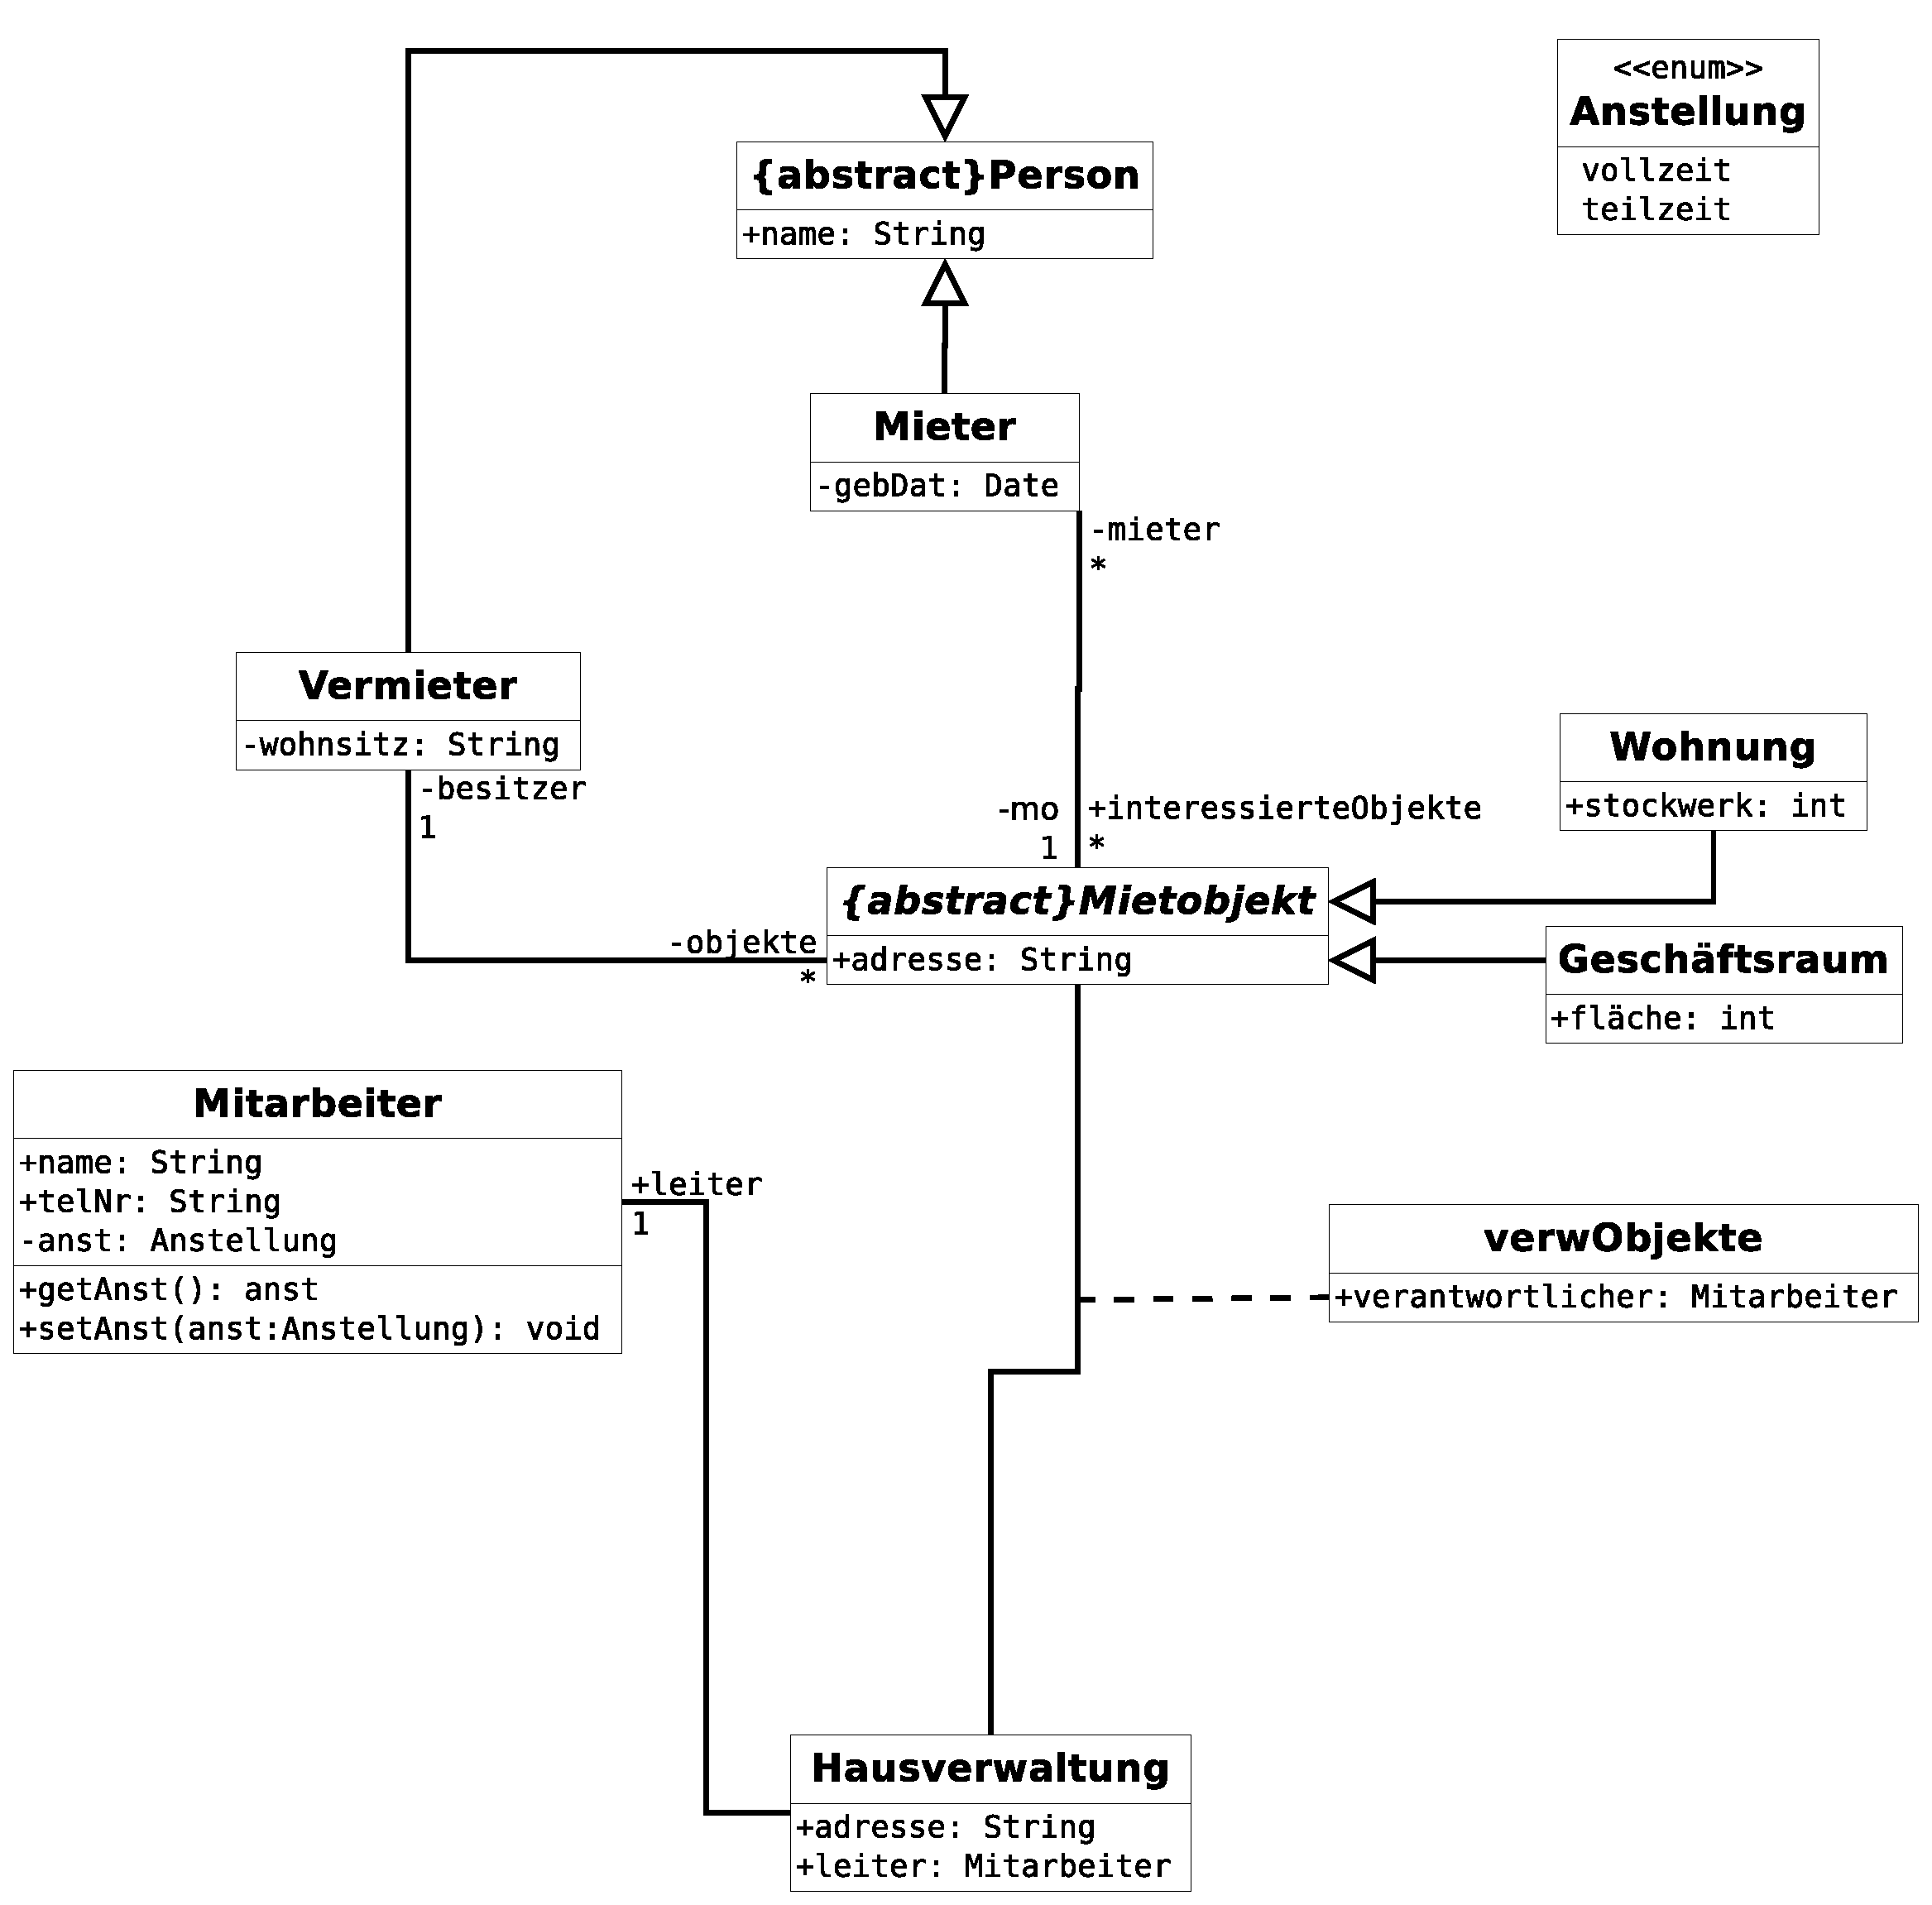
\includegraphics[scale=0.4]{Aufgabe3.eps}
    \end{center}
    
  \end{solution}

\newpage

% AUSSTÄNDIG
  \problemnumber{4}
  \begin{problem}
    Von jedem Konzert werden das Datum sowie der Veranstaltungsort gespeichert. Weiters wird vermerkt, um
welche Musikgenres bei dem Konzert vertreten sind. Dabei gibt es Klassik, Rock, Pop und Heavy Metal. Auf
einem Konzert können mehrere Bands spielen, die wiederum auf mehreren Konzerten spielen können. Dabei
wird die Höhe der Gage, die eine Band für einen Auftritt erhält, gespeichert. Für eine Band speichern wir deren
Namen sowie deren Musikgenre. Von Personen speichern wir deren Namen. Es gibt zwei Arten von Personen,
Musiker und Manager. Von Musikern vermerken wir zusätzlich deren Künstlernamen und von Managern deren
Telefonnummer. Ein Musiker kann in mehreren Bands spielen welche wiederum aus mehreren Musikern bestehen
kann. Für die Zugehörigkeit eines Musikers zu einer Band speichern wir das von ihm gespielte Instrument.
Eine Band wird von genau einem Manager betreut und ein Manager kann mehrere Bands betreuen. Für ein
Musikstück speichern wir dessen Titel und Länge in Sekunden. Auf einem Konzert kann ein Musikstück von
höchstens einer Band gespielt werden. Jedoch kann eine Band auf einem Konzert mehrere Musikstücke spielen.
Weiters kann ein Musikstück von einer Band auf mehreren Konzerten gespielt werden.
  \end{problem}
  \begin{solution}\hfill

    \begin{center}
      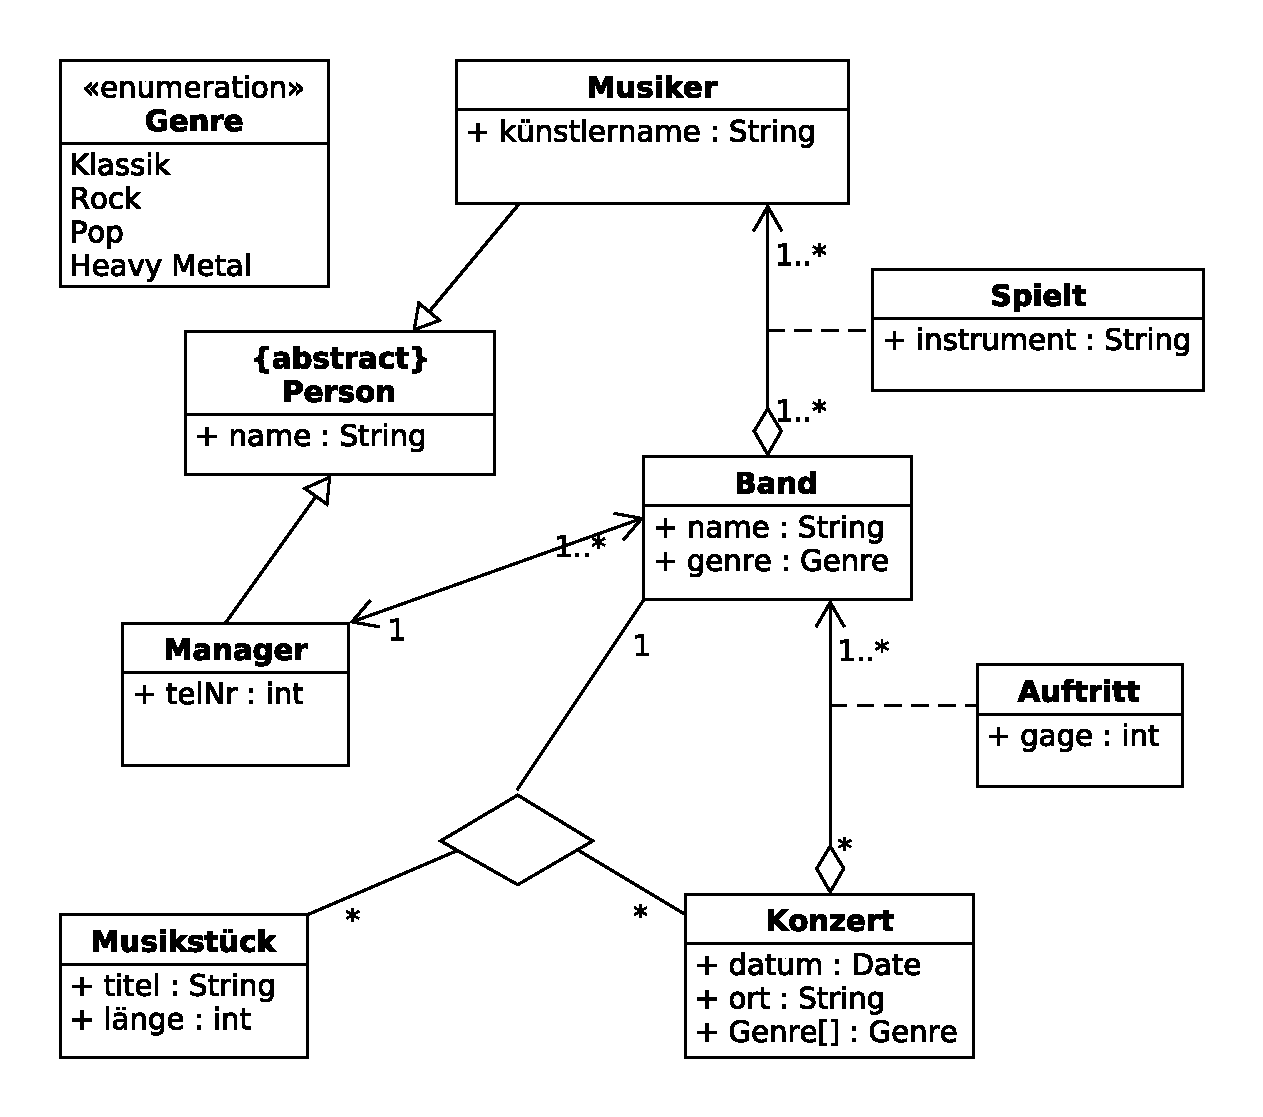
\includegraphics[scale=0.7]{Aufgabe4.eps}
    \end{center}
  \end{solution}


% AUSSTÄNDIG
  \problemnumber{5}
  \begin{problem}
    Bilden Sie die folgenden Sachverhalte mit einem Klassendiagramm ab:
Von Politikern speichern wir Name und Geburtsdatum. Jeder Politiker ist Mitglied von genau einer Partei. Eine
Partei kann wiederum mehrere Politiker als Mitglieder haben. Von Parteien speichern wir deren Bezeichnung
sowie deren Kürzel. Jede Partei hat einen Obmann der Politiker ist. Von einem Nationalrat speichern wir den
Zeitpunkt dessen Bestellung. Ein Nationalrat hat genau 183 Abgeordnete die Politiker sind. Von jedem dieser
Abgeordneten erfassen wir dessen Gehalt. Ein Politiker kann in mehreren Nationalräten bestellt sein. Weiters
hat ein Nationalrat genau drei Politiker die Nationalratspräsidenten sind. Ein Politiker kann in höchstens zwei
Nationalräten als Präsident fungieren. Für jeden dieser Präsidenten speichern wir ob der Präsident erster, zweiter
oder dritter Nationalratspräsident ist.

Erweitern Sie das Klassendiagramm aus Aufgabe 5 wie folgt:
Von einer Regierungsfunktion speichern wir deren Gehalt. Es gibt zwei verschiedene solche Funktionen, Minister und Bundeskanzler. Von der Funktion Minister erfassen wir zusätzlich das zugewiesene Ressort und für
die Funktion Bundeskanzler erfassen wir die Adresse der Amtswohnung. Staatssekretäre sind formell nicht eine
Regierungsfunktion, jedoch wollen wir auch diese Positionen als solche modellieren. Wir speichern von dieser
Funktion zusätzlich eine Beschreibung der Aufgaben. Ein Minister und der Bundeskanzler haben höchstens
einen Staatssekretär zugeordnet. Ferner ist ein Staatssekretär entweder einem Minister oder dem Bundeskanzler
zugeordnet. Von einer Regierung speichern wir den Zeitpunkt der Bestellung sowie den Typ der Regierung.
Hierbei gibt es Minderheitsregierungen, Alleinregierungen und Koalitionsregierungen. Ein Politiker kann eine
Regierungsfunktion in mehreren Regierungen übernehmen. Weiters kann in einer Regierung eine Regierungs-
funktion von bis zu zwei Politikern übernommen werden. Umgekehrt kann ein Politiker in einer Regierung
mehrere Funktionen übernehmen.
  \end{problem}
  \begin{solution}\hfill
    \begin{center}
      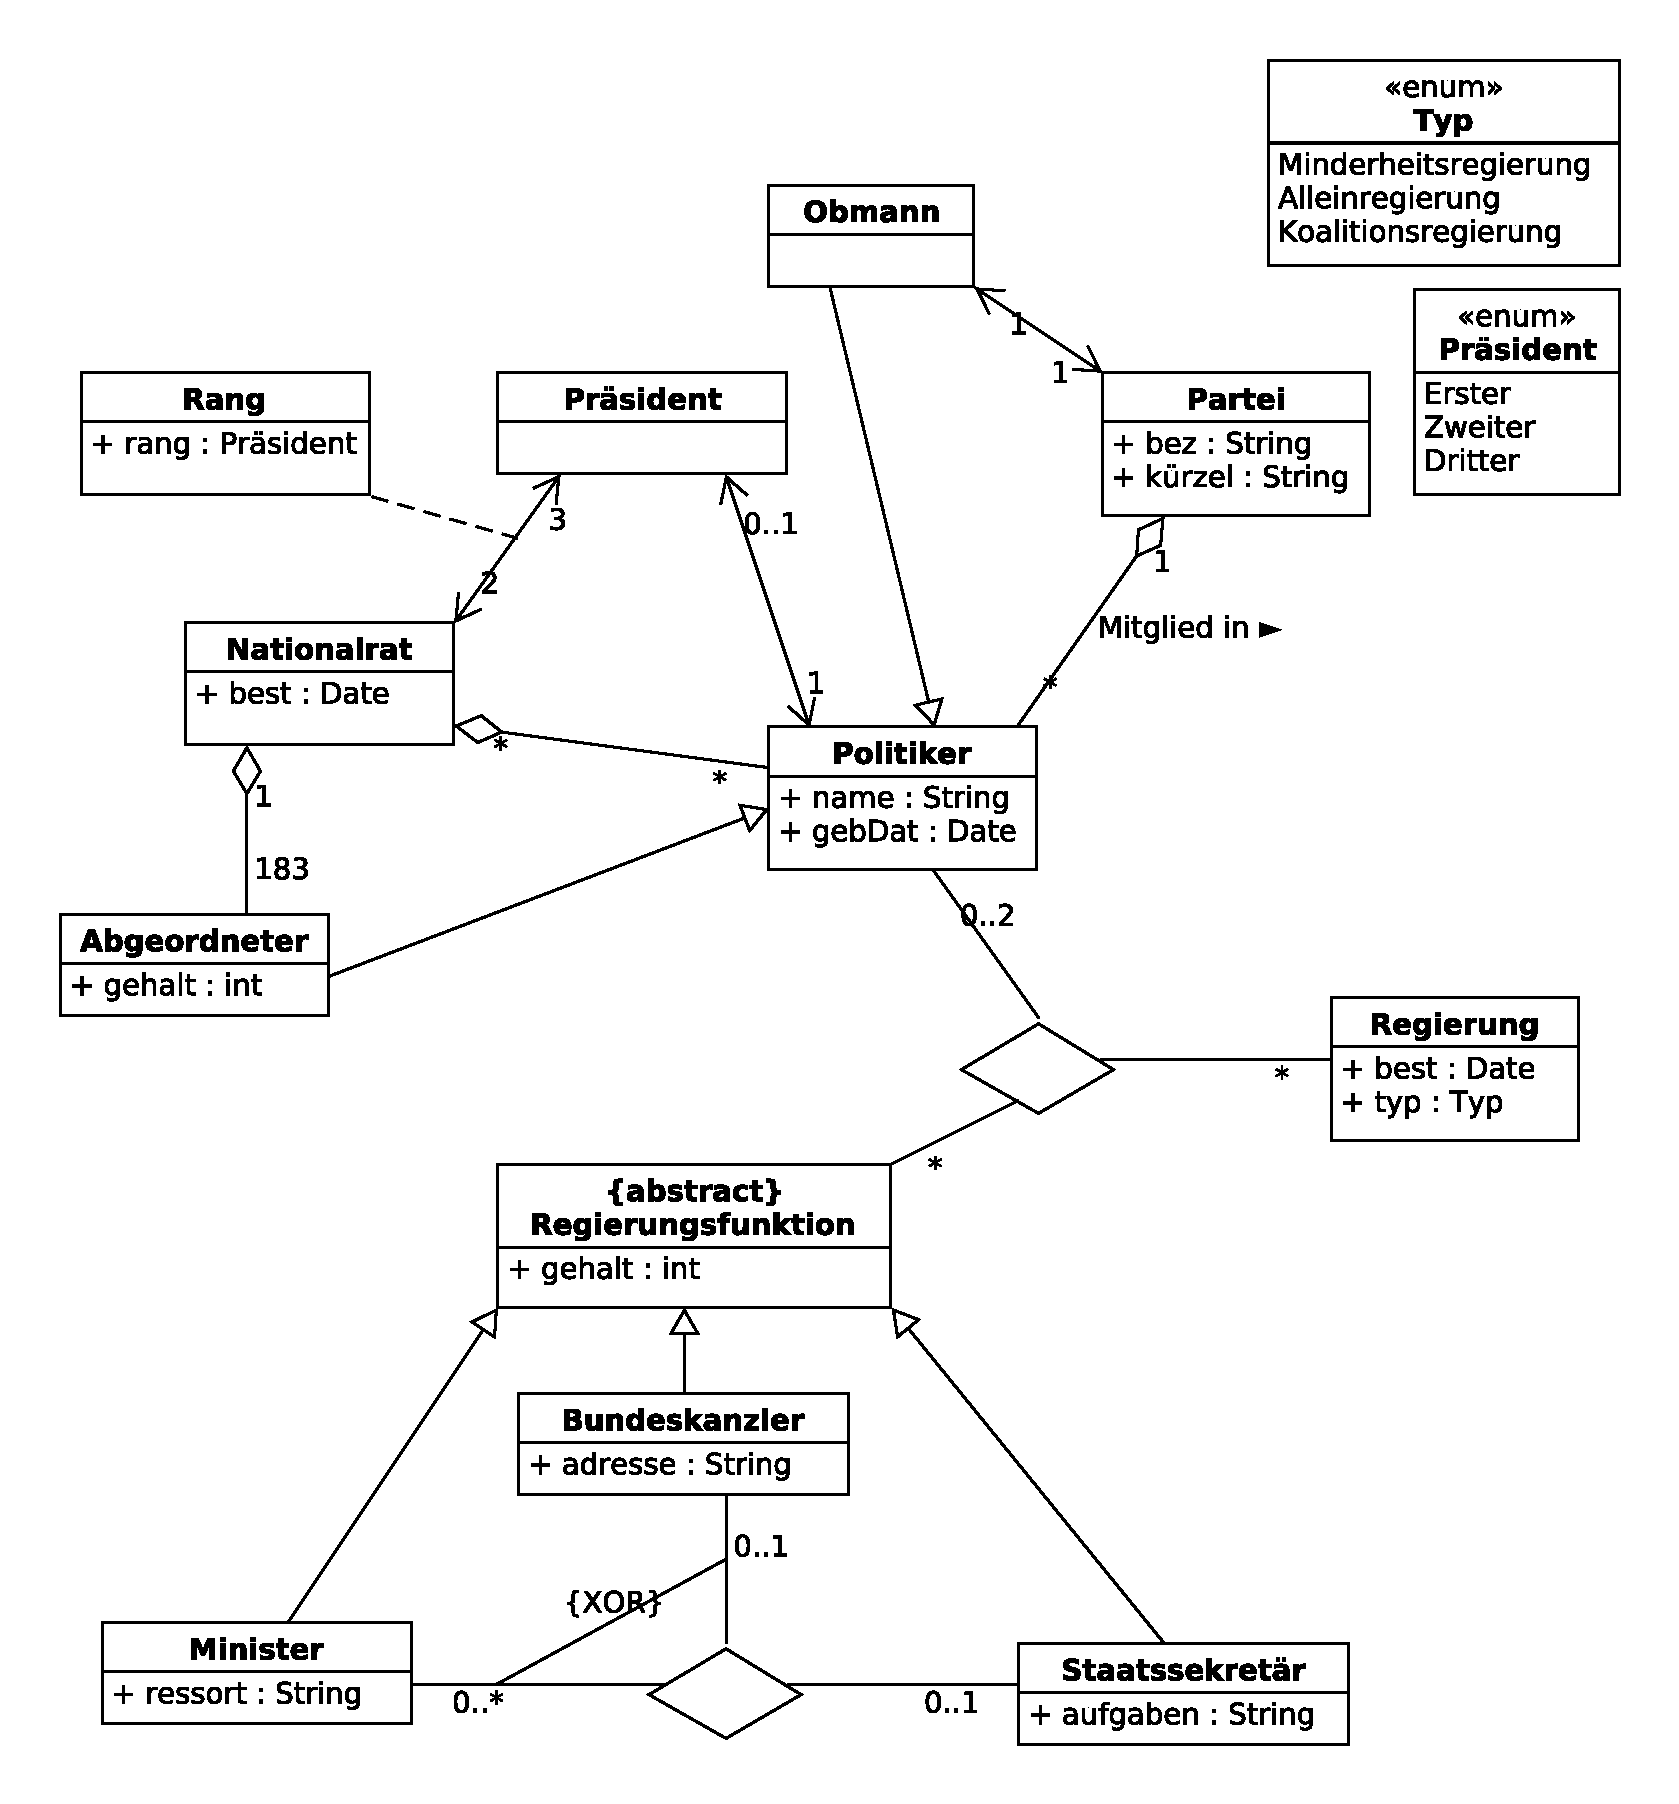
\includegraphics[scale=0.3]{Aufgabe5u6.eps}
    \end{center}
  \end{solution}


\end{document}